\documentclass[10pt,journal,letterpaper,compsoc]{IEEEtran}
\makeatletter
\def\markboth#1#2{\def\leftmark{\@IEEEcompsoconly{\sffamily}\MakeUppercase{\protect#1}}%
\def\rightmark{\@IEEEcompsoconly{\sffamily}\MakeUppercase{\protect#2}}}
\makeatother

%\documentclass[prodmode,acmtecs]{acmsmall}
%\pdfpagewidth=8.5in
%\pdfpageheight=11in

\usepackage[latin1]{inputenc}	% for Latin languages
\usepackage[T1]{fontenc}	% for ISO and UTF characters
\usepackage[english]{babel}	% for multilingual support
\usepackage{graphicx}
\usepackage{multirow}
\usepackage{stfloats}
\usepackage{booktabs}
%\usepackage[caption=false]{caption}
\usepackage[caption=false,font=normalsize,labelfont=sf,textfont=sf]{subfig}
\usepackage{color}
\definecolor{Red}{rgb}{.9,0,0}

%\newcommand{\codefont}{\footnotesize\sffamily}
\newcommand{\codefont}{\scriptsize\sffamily}

\usepackage{listings}
%\lstset{keywordstyle=\bfseries, flexiblecolumns=true, breaklines = true, numbers = left}
\lstset{keywordstyle=\bfseries, flexiblecolumns=true, breaklines = true, numbers = none}
\lstloadlanguages{[ANSI]C++,HTML}
\lstdefinestyle{prg} {basicstyle=\codefont, lineskip=-0.2ex, showspaces=false}

\usepackage{microtype}

\usepackage{hyperref}
\hypersetup{
    colorlinks=false,
    pdfborder={0 0 0},
}


\newcommand{\fig}[4][htbp]{
  \begin{figure}[#1] {\centering\scalebox{#2}{\includegraphics{fig/#3}}\par}
    \caption{#4\label{#3}}
  \end{figure}
}

\newcommand{\multfigtwoh}[6][htbp]{
\begin{figure*}[#1]
  \centering
  \subfloat[]{\label{#3}\scalebox{#2}{\includegraphics{fig/#3}}}
  \subfloat[]{\label{#4}\scalebox{#2}{\includegraphics{fig/#4}}}
  \caption{#6}
  \label{#5}
\end{figure*}
}

\newcommand{\multfigtwov}[6][htbp]{
\begin{figure}[#1]
  \centering
  \subfloat[]{\label{#3}\scalebox{#2}{\includegraphics{fig/#3}}}\\
  \subfloat[]{\label{#4}\scalebox{#2}{\includegraphics{fig/#4}}}
  \caption{#6}
  \label{#5}
\end{figure}
}

\newcommand{\figR}[5][htbp]{
  \begin{figure}[#1]{\centering\scalebox{#2}{\includegraphics[angle=#5]{fig/#3}}\par}
    \caption{#4\label{#3}}
  \end{figure}
}

\newcommand{\figTC}[4][htbp]{
  \begin{figure*}[#1] {\centering\scalebox{#2}{\includegraphics{fig/#3}}\par}
    \caption{#4\label{#3}}
  \end{figure*}
}

\newcommand{\figEMPTY}[5][htbp]{
  \begin{figure}[#1]
    \fbox{\begin{minipage}{#2}\hfill\vspace{#3}\end{minipage}}
    \centering
     \label{#4}
    \caption{#5}
  \end{figure}
}

\newcommand{\tab}[3][htbp]{
  \begin{table}[#1]
    \footnotesize
    \centering
    \caption{#3}
    \include{tab/#2}
    \label{#2}
  \end{table}
}

\newcommand{\tabTC}[3][htbp]{
  \begin{table*}[#1]
    \footnotesize
    \centering
    \caption{#3}
    \include{tab/#2}
    \label{#2}
  \end{table*}
}

 %new commands 

\hyphenation{in-ter-face}

\newcommand*\condhwsw{\scalebox{0.5}{
\includegraphics{fig/fig_hw_sw_scenarios_cond_inhe_symbol}}}

\newcommand*\inherit{\scalebox{0.5}{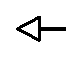
\includegraphics{fig/fig_inheritance_symbol}}}

%\setlength{\intextsep}{8pt}
%\setlength{\floatsep}{8pt}
%\setlength{\dblfloatsep}{8pt}
%\setlength{\abovecaptionskip}{3pt}
%\setlength{\belowcaptionskip}{1pt}
%%%%%
%\setlength{\intextsep}{-1ex} % remove extra space above and below in-line float
%Options    
%\floatsep - Space between floats. \dblfloatsep for 2 column format
%\intextsep - Space above and below in-line text floats
%\abovecaptionskip - Space above float caption
%\belowcaptionskip - Space below float caption
%%%%%%
%\raggedbottom

\begin{document}

%\markboth{T. R. M�ck and A. A. Fr�hlich}{Unified Design of Hardware and Software Components}

\title{Towards Unified Design of Hardware and Software Components Using C++}

\author{Tiago~Rog�rio~M�ck,~\IEEEmembership{Member,~IEEE,}
        and~Ant�nio~Augusto~Fr�hlich,~\IEEEmembership{Member,~IEEE,}%
%\author{Tiago~Rog�rio~M�ck~and~Ant�nio~Augusto~Fr�hlich%
\IEEEcompsocitemizethanks{\IEEEcompsocthanksitem T. R. M�ck and A. A. Fr�hlich are with the
Software/Hardware Integration Lab , Federal University of Santa Catarina,
Florian�polis, Brazil.\protect\\
E-mail: \{tiago,guto\}@lisha.ufsc.br}% <-this % stops a space
\thanks{}}

%\author{Authors omitted for peer review}

\markboth{IEEE Transactions on Computers,~Vol.~x, No.~x, Month~year}%
{Shell \MakeLowercase{\textit{et al.}}: Unified Design of Hardware and Software Components}

\IEEEpubid{\makebox[\columnwidth]{\hfill 0000--0000/00/\$00.00~\copyright~2013 IEEE}%
\hspace{\columnsep}\makebox[\columnwidth]{Published by the IEEE Computer Society\hfill}}


\IEEEcompsoctitleabstractindextext{%
\begin{abstract}
The increasing complexity of current embedded systems is pushing their design to higher levels of
abstraction, leading to a convergence between hardware and software design methodologies. In this
paper we aim at narrowing the gap between hardware and software design by introducing a strategy
that
handles both domains in a unified fashion. We leverage on \emph{aspect-oriented programming} and
\emph{object-oriented programming} techniques in order to provide \emph{unified} C++ descriptions of
embedded system components. Such unified descriptions can be obtained through a careful design
process focused on isolating aspects that are specific to hardware and software scenarios. Aspects
that differ significantly in each domain, such as resource allocation and communication,
were isolated in \emph{aspect programs} that are applied to the unified descriptions
before they are compiled to software binaries or synthesized to dedicated hardware using
\emph{high-level synthesis} tools. Our results show that our strategy leads to reusable and flexible
components at the cost of an acceptable overhead when compared to software-only C/C++ and
hardware-only C++ implementations.
\end{abstract}
\begin{keywords}
System-level design, HW/SW co-design, High-level synthesis, Aspect-oriented system design.
\end{keywords}}

\maketitle

\section{Introduction}
\label{sec:introduction}

Embedded systems are becoming increasingly complex as the advances of the semiconductor industry
enable the use of sophisticated computational resources in a wider range of applications. Depending
on the application's requirements (e.g. performance, energy consumption, cost, etc.), the
development of such systems may encompass an integrated hardware and software design that can be
realized by several different architectures, ranging from simple 8-bit microcontrollers to
complex \textit{multiprocessor system-on-chips}~(MPSoCs).

In order to deal with this complexity, embedded system designs are being pushed to the
\emph{system-level}. In this scenario, a convergence between hardware and software design
methodologies is desirable, since a unified modeling approach would enable one to take decisions
about hardware/software partitioning later in the design process, maybe even automatically. In the
last few years, advances in \textit{electronic design automation}~(EDA) tools
are allowing hardware synthesis from high-level, software-like descriptions. This process is known
as \textit{high-level synthesis}~(HLS) and allows designers to describe hardware components using
languages like C++, and higher-level techniques, such as \textit{Object-Oriented Programming}~(OOP).
The focus of these tools~\cite{Calypto:Catapult,Forte:Cynthesizer,Xilinx:AutoESL},
however, is hardware synthesis, and they do not provide a clear design methodology for developing
components which could be implemented as both hardware and software.

Aiming to narrow this gap, in this paper we
describe some design guidelines and mechanisms which support the implementation of both hardware and
software components from a single, unified, C++ description. Our guidelines are built upon the
\textit{Application-driven Embedded System Design}~(ADESD) methodology~\cite{Polpeta:2005}. ADESD
leverages on OOP and \textit{aspect-oriented programming}~(AOP) concepts, defining a domain
engineering strategy which allows us to clearly separate the core behavior and the structure of a
component from aspects that must be handled differently whether a component is implemented as
hardware or software. Such specific characteristics are modeled in special constructs called
\emph{aspects} and are applied to the unified descriptions of components only after the
hardware/software partitioning is defined, yielding the final implementation in the target domain
(hardware or software). In order to generate descriptions that can be efficiently synthesized by
HLS tools or compiled to a software binary, the implementation of both the components and the
mechanisms which adapt them make extensive use of C++ \emph{generative
programming}~\cite{Czarnecki:2000} techniques such as \emph{static metaprogramming}. To evaluate the
efficiency of our approach, we present the implementation of a \textit{Private Automatic Branch
Exchange}~(PABX) SoC of which some components were implemented using our unified design strategy.

It is important to recall that it is not a goal of this work to discuss the quality of hardware
implementation generated using HLS tools, neither the intrinsic differences between software and
hardware that cannot yet be fully handled by such tools. We take in consideration the fact that
these tools impose limitations to source descriptions (such as dynamic allocation and binding). As
it will be demonstrated in the following sections, limitations of this kind can be circumvented by
our unified approach.

The remaining of this paper is organized as follows: Section \ref{sec:related_work} presents a
discussion about works related to the integration of the hardware and software design flows; Section
\ref{sec:background} presents an overview of previous contributions upon which this work is built;
in Sections \ref{sec:proposal} and \ref{sec:implementation}  we discuss the characteristics that are
part of software and hardware scenarios and present our approach for their proper separation and
implementation; Section \ref{sec:case_study} describes our case studies and shows our experimental
results; and Section \ref{sec:conclusion} closes the paper with our conclusions.

\section{Related work}
\label{sec:related_work}

Several design methodologies and tools were proposed in order to provide more tightly coupled
hardware and software design flows. Most of these methodologies are based on the concept of building
a system by assembling pre-validated components. The \textit{Ptolemy extension as a Codesign
Environment}~(PeaCE)~\cite{Ha:2008}, an extension of the Ptolemy project~\cite{Eker:2003}, is a
synthesis framework for real-time multimedia applications. PeaCE takes models composed by
synchronous data-flow graphs and extended \textit{finite state machines}~(FSMs) and either generates
C code or maps the models to
pre-existing IP cores and processors. ROSES~\cite{Dziri:2004} is a design flow which automatically
generates hardware, software, and interfaces from an architectural model of the system and a library
of pre-validated components. The \emph{Metropolis} and its successor
\emph{Metro-II}~\cite{Davare:2007} follow the \emph{Platform-based
design}~(PBD)~\cite{Vincentelli:2001} methodology. They propose the use of a metamodel with formal
semantics to capture designs. An environment to support simulation, formal analysis, and synthesis
is also provided. Despite providing integration frameworks for the entire design flow, these
methodologies do not define clear guidelines to design new reusable components. Also, mapping the
application model to pre-existing components limits hardware/software partitioning.
%Also in PDB the hardware/software partitioning must be defined in the early design stages and is
%limited by the platform specification. 

In order to overcome these limitations, one must focus on closing the \emph{design gap} of software and
hardware components. State-of-the-art EDA tools (e.g. Calypto's CatapultC~\cite{Calypto:Catapult},
Forte's Cynthesizer~\cite{Forte:Cynthesizer}, Xilinx's AutoESL~\cite{Xilinx:AutoESL}) support
hardware synthesis from high-level C++/C-based constructs. Indeed, several works have already
demonstrated the  applicability of HLS for implementing hardware
components such as signal processing filters, cryptographic cores, and other computationally
intensive components~\cite{Cong:2011}. Our aims are different however. We want to describe
components in a high level of abstraction, but those should be implementable in hardware as well as
in software, and with performance close to software-only and hardware-only implementations. 

%maybe include figures of the other flows
On this track, the OSSS+R methodology~\cite{Schallenberg:2009} raises
the level of \textit{register transfer level}~(RTL) SystemC by adding new language constructs to
support synthesizable polymorphism and high-level communication. However, hardware/software
partitioning must still be done in the beginning of the design process, and the
inclusion of non-standard language constructs reduces the compatibility of the design with available
compilers and hardware synthesis tools. The \emph{Saturn}~\cite{Mischkalla:2010} design
flow also contributes in this scenario, but follows a different approach. It aims to close the gap
between UML-based modeling and the execution of the models for their verification.
The authors have
elaborated over \emph{SysML}, an extension of UML for system-level design, and
developed a tool which generates C++ for software and RTL SystemC for hardware. Although using a
single language, software and hardware are still modeled separately. Additionally, it is not clear
whether their tool generates code only for the interface and integration of components, or the
behavior is also inferred from the SysML models.

SystemCoDesigner~\cite{Keinert:2009} is a tool which integrates a HLS flow with design space
exploration. The design entry of SystemCoDesigner is an actor-based data flow model whose actors can
be converted to synthesizable SystemC or to C++ for software compilation. However, as the authors
themselves claim, SystemCoDesigner targets mostly data-flow-based applications, and they do not
provide directions towards a more general deployment. The System-on-chip
environment~(SCE)~\cite{Rainer:2008} takes SpecC models as input and provides a refinement-based
tool flow.  Guided by the designer, the SCE automatically generates a set of
\textit{Transaction-level models}~(TLM) that are further refined to pin- and 
cycle-accurate system implementation.

Other works focus mainly on the interface between software and hardware. For instance, 
the ReconOS~\cite{Lubbers:2008} and the BORPH operating
system~\cite{So:2008} provide a unified interface for both domains. In these works a task performed
in hardware is seen with the same semantics as a software thread, and a system call interface is
provided to hardware components. However, despite providing this unified interface, they do not
cover the gap that still exists between the way the hardware and software threads themselves are
implemented. The work of \textit{Rinc�n et al}~\cite{Rincon:2009} is based on concepts from
distributed object platforms such as CORBA and Java RMI and provides a tool which generates the
communication glue necessary so that hardware and software components can communicate seamlessly.


\section{Application-driven Embedded System Design}
\label{sec:background}

The \textit{Application-driven Embedded System Design}~(ADESD) methodology~\cite{Polpeta:2005}
elaborates on the \emph{Object-Oriented Decomposition}~\cite{Booch:2007} strategy to add the concept
of \emph{aspect}
identification and separation at early stages of design. Variability analysis, as carried out in
object-oriented decomposition, does not emphasizes the differentiation of variations that belong to
the basic behavior of a component from those that emanate from the execution scenarios being
considered for it. Components that incorporate environmental dependencies have a smaller chance of
being reused in new scenarios, and, given that an application-driven system will be confronted
with a new scenario virtually every time a new application is defined, allowing such dependencies
could severely hamper the system.

Nevertheless, one can reduce such dependencies by applying the key concept of \emph{aspect-oriented
programming}~(AOP)~\cite{Kiczales:1997}, i.e. aspect separation, to the decomposition process.
Scenario dependencies can be encapsulated in special constructs called \emph{aspects}. An aspect
weaving semantic is then defined to describe when and how aspects are applied to components. By
doing so, one can tell variations that shape new components from those that yield scenario aspects.
For instance, instead of modeling a new component for a family of communication mechanisms that is
able to operate in the presence of multiple threads, one could model multithreading as a scenario
aspect that, when activated, would lock the communication mechanism (or some of its operations) in a
critical section.  

The aspect weaving semantics in ADESD is defined by constructs called \emph{Scenario
adapters}~\cite{Mueck:OSR:2012}. Scenario adapters were developed around the idea of components
getting in and out of an execution scenario, allowing actions to be executed at these points.  These
actions may take place respectively before and after each of the component's operation in order
to setup the conditions required by the scenario. 
%Figure \ref{fig_scenario_adapter} shows the
%general structure of a scenario adapter. A \emph{Scenario} construct represents the execution
%scenario and aggregates all aspect programs that characterize it. The scenario adapter
%then applies the scenario to the target component. 
As can be seen in the following sections,
scenario adapters can be fully implemented in C++ using its OOP and template metaprogramming
capabilities\footnote{this paper assumes prior knowledge about OOP, UML and C++. The reader may
refer to \cite{Larman:2005}, \cite{Czarnecki:2000}, and \cite{Andrei:2001} for an indepth
explanation of the relevant concepts}. In contrast to traditional aspect weaving
approaches, such as AspectC++~\cite{Spinczyk:2002}, scenario adapters do not require external
tool support and can be compiled by any standard C++ compiler. 

%\figSC{.6}{fig_scenario_adapter}{Component adaptation using a scenario adapter.}

\subsection{ADESD for HW/SW design}
\label{sec:background:adesd_hw_sw}

In ADESD, knowledge about implementation details should be driven to identify and isolate
scenario aspects. In general, aspects such as identification, sharing, authentication,
and encryption can be represented as scenario aspects. Such aspects are part of the
\emph{application domain}, since they describe behavior related to the application functional
requirements. However, the design of new components in a HLS-capable system-level environment must
also take into considerations the \emph{platform domain}, therefore yielding at least two additional
scenarios: a \emph{software scenario}, in which the component is deployed as part of the software
running in a processor; and a \emph{hardware scenario}, in which the component is deployed as dedicated
hardware.

An initial work~\cite{Pizani:2011} has already shown how the ADESD methodology was used to provide a
C++ description of a resource scheduler suitable for high-level hardware synthesis. In this paper we
further extend the previous case in order to show how ADESD's aspect separation mechanisms can be
used to yield components susceptible to both hardware and software synthesis. We demonstrate how
characteristics specific of a hardware or a software scenario can be isolated from the core behavior
and the interface of a component. By following our design guidelines, the same component description
can be tailored by the scenario adapter in order to feed either a software compilation flow or a
hardware HLS flow.

         
\section{Unified hardware/software design}
\label{sec:proposal}

%To save space, this paragraph can be removed or merged with the next one
HLS tools allow for hardware synthesis from algorithms described in languages such as C++. When
aiming at this goal, the implementation of the algorithm itself is usually very similar to what is
seen in software. However, at component level, several characteristics arise which distinguish
descriptions aiming at hardware and software. In the following sections we first discuss these
differences. Then, we present our strategy for the separation of hardware and software concerns and
how we have achieved unified C++ descriptions.

%This subsection can be merged with the top-level one if the above paragraph is removed
\subsection{Differences between hardware and software}
\label{sec:proposal:hw_sw_differences}

Table \ref{tab_comm_interface} summarizes the most common component communication patterns. 
In the software domain, components may be objects which communicate using method invocation
(considering an OOP-based approach), while in the hardware domain, components communicate using
input/output signals and specific handshaking protocols. For communication through different
domains, the software must provide appropriate \textit{hardware abstraction layers}~(HAL) and
\textit{interrupt service routines}~(ISR), while the hardware must be aware that it is requesting a
software operation.

\tabSC[ht]{tab_comm_interface}
{Usual component communication patterns. The \emph{Caller} requests operations from the
\emph{Callee}.}

Another concern is related to the composition of hardware/software components in an
object-oriented model and the mapping of high-level components to physical implementations. Figure
\ref{fig_oop_to_phy} shows a simple system modeled using such strategy and illustrates two different
mappings. In OOP, the original structure may be ``disassembled'' in the final physical implementation if different
objects in the same class hierarchy represent components that are to be implemented in different
domains. For example, \emph{C2} is ``inside'' \emph{C1} in the OO model in Figure
\ref{fig_oop_to_phy}, but, in a possible final implementation, \emph{C2} could be implemented as a
hardware component while \emph{C1} could run as software in a processor (first mapping in Figure
\ref{fig_oop_to_phy}). 

\figSC{.6}{fig_oop_to_phy}{Possible mappings of an object-oriented model to physical
implementations}

When focusing on an OOP-based methodology, one must provide ways to make these different mapping
transparent to the designer. Furthermore, the different communication patterns between hardware and
software must also be properly abstracted. For instance, in the second mapping shown in Figure
\ref{fig_oop_to_phy}, \emph{C1} can call \emph{C2}'s methods directly, while in the first mapping
a hardware/software communication mechanism must be defined. In this sense, the method call interface
must also be properly adapted when a component is to be implemented in hardware, so it can be compliant 
with HLS tools requirements. In Calypto's CatapultC~\cite{Calypto:Catapult} and Xilinx's 
AutoESL~\cite{Xilinx:AutoESL}, for instance, the top-level interface of the resulting hardware
block (port directions and sizes) is inferred from the signature of a \emph{single
function}\footnote{both tools also allow the specification of the entry point as a SystemC module
with signal ports defining the IO protocol}.

Another important characteristic that distinguishes hardware from software is resource allocation.
The hardware is frozen and common software features, such as dynamic resource allocation, are not
easily available. Therefore, in code suitable for hardware synthesis, all data structures must
reside in statically allocated memory. Some works focus on this problem by relying on dynamic
reconfiguration technologies of FPGAs to support hardware components instantiation at
run-time\cite{Abel:2010}. However, this is not the focus of our current work. We aim at providing
more general guidelines for describing components.

\subsection{Defining C++ unified descriptions}
\label{sec:proposal:unified_design}

C++ code unified and suitable for automatic implementation in both hardware and software must
follow a careful design process so it will not contain characteristics specific of hardware or
software. In this sense, the goal of this section is to demonstrate how the
application-oriented design process proposed by ADESD yields designs that allow such concerns to be
handled externally and implemented as aspect programs. To illustrate our design process, 
we describe in more details one of our case studies: the design
and unified implementation of the EPOS's thread scheduler. The
\textit{Embedded Parallel Operating System}~(EPOS)~\cite{EPOS:2011} is a case study on which the
design artifacts proposed by ADESD were implemented and validated. The complex behavior of the
scheduler motivated its choice as our main case study. Task scheduling involves both
synchronous (e.g. creating a new thread) and asynchronous (e.g. preempting the execution of another
component) operations. Furthermore, enabling a hardware/software scheduler allows a system with
less jitter and better support for real-time applications~\cite{Marcondes:2009:2}. Figure
\ref{fig_epos_scheduler} shows the entities identified in the domain of real-time scheduling. 

\figSC{.6}{fig_epos_scheduler}{Simplified UML class diagram of scheduling-related classes in EPOS.}

In this domain decomposition, a task is represented by the class \emph{Thread} which defines the execution flow
of the task, implementing the traditional functionality of such kind of abstraction (e.g. timing
interrupt handling and context switching). Concerns such as timing management are performed
through OS abstractions for CPU-dependent hardware (e.g. the \emph{Timer} class). 

The classes \emph{Scheduler} and \emph{Criterion} define the structure that realizes the task
scheduling itself. Traditional implementations of scheduling algorithms are usually done
by a hierarchy of specialized classes of an abstract \emph{Scheduler} class, which can be further
specialized to bring new scheduling policies to the system. In order to reduce the complexity of
code maintenance (generally present in such hierarchy of specialized classes), as well as to
promote its reuse, our design detaches the scheduling policy from its mechanisms (lists
implementations) and also detaches the scheduling policy from the thread it represents. The 
separation of the mechanism from the scheduling policy is what in fact allows the deployment of the
scheduler as both hardware and software. The unified description of the \emph{Scheduler} component
implements only the mechanisms that realize the ordering of the tasks, based on the selected policy.
In this sense, the same component can realize distinct policies, as the definition of the policy
is confined in the \emph{Criterion} component, which isolates the comparison algorithm between the
elements of the scheduler queue.

\subsubsection{Scheduler implementation}
\label{sec:proposal:unified_design:sched}

According to such decomposition, the scheduler must be implemented in a flexible way to enable the
decoupling of the policy and the resource from the scheduling mechanisms. To achieve such
flexibility without imposing performance penalties, the implementation of the scheduler itself
makes extensive use of \emph{static metaprogramming techniques}~\cite{Czarnecki:2000}. Figure
\ref{fig_epos_scheduler_extended_full} shows a more detailed definition of the scheduler. The
component is actually defined through the class template \emph{Scheduler<T>}, which receives the
type of the resource being scheduled as template parameter (in this case, an object of the type
\texttt{Thread}).

The \emph{List}\inherit\emph{Ordered\_List} class hierarchy in Figure
\ref{fig_epos_scheduler_extended_full} defines a linked list used to implement the scheduling queues.
An important aspect in this implementation lies in the fact that the linking and storage concerns
are factored and implemented separately, while static metaprogramming is used to integrate these
concerns at compile-time. That is, the list classes are not responsible for the allocation of memory
for the internal nodes and the objects it stores. They implement only the list algorithms and deal
with references to such elements. The motivation for this approach is to avoid the excessive
allocation/deallocation of nodes when the same object is repeatedly inserted and then removed from
the list, which tends to happen frequently in a thread scheduling environment. As can be seen in
Section \ref{sec:proposal:aspects}, this separation of concerns also allows us to handle memory
allocation as a separated aspect according to the target implementation scenario.

\figSC{.6}{fig_epos_scheduler_extended_full}{Definition of the Scheduler component}

As can be seen in Figure \ref{fig_epos_scheduler_extended_full}, a node for the list is defined by the
class template \emph{Scheduling\_Element<T,Rank>}. The \emph{Rank} parameter defines the
ordering criterion and maps directly to one of the criteria shown on Figure
\ref{fig_epos_scheduler} (\emph{Rank} is also a parameter for the class
\emph{Scheduling\_List}). \emph{Scheduler} then inherits from \emph{Scheduling\_List},
defining \emph{Scheduling\_Element} as the type for list nodes and 
\emph{Traits<Scheduler<T> >::Criterion} as the ordering criterion. The criterion depends on
static configurations defined in template classes called \emph{Traits}~\cite{Myers:1995}. In Figure
\ref{fig_epos_scheduler_extended_full}, when the scheduler is used with the class \emph{Thread},
\emph{Traits<Scheduler<T> >} maps to \emph{Traits<Scheduler<Thread> >}, which can be defined as
follows:
%
\progcppinline{code_traits_sched}
%
Trait classes provide a convenient way to associate related types, values, and functions with a
template parameter type without requiring their definition as members of the
type~\cite{Myers:1995}. 


\subsubsection{Scheduler implementation for HW/SW}
\label{sec:proposal:unified_design:hw_sw_sched}

%Mapping pointers in a synthesizable C++ to memory access in the software address space could be
%supported using libraries that require some customization at the RTL, like the one provided by
%ReconOS~\cite{Lubbers:2008}.

Current HLS tools support ANSI C++ and allow the use of advanced language constructs, such as
pointers, classes, arrays, and template metaprogramming. Therefore, the core scheduling algorithm
and the class hierarchy shown previously required only minor modifications so it could serve as
input for both hardware and software implementation flows. However, as mentioned in section
\ref{sec:proposal:hw_sw_differences}, the \emph{communication interface} and \emph{resource
allocation} must be handled differently whether a component is implemented as hardware or software.
Figure \ref{fig_epos_scheduler_wrapped} gives an overview of the resulting final implementations
that incorporate these concerns.

\multfigtwov{.6}
{fig_epos_scheduler_wrapped_hw}{Hardware component}
{fig_epos_scheduler_wrapped_sw}{Software component}
{fig_epos_scheduler_wrapped}{Scheduler implemented in both hardware and software}

As mentioned in section \ref{sec:proposal:unified_design:sched}, the allocation of list nodes is
not part of the core implementation of the scheduler. However, to implement the scheduler as a
self-contained component in hardware, an \emph{allocation management} block was defined separately
and associated to the scheduler in order to keep the linked list node in the same ``synthesis
scope'' of the final component. This was necessary since pointers to, for instance, memory locations
allocated in software would not make sense in the scope of a self-contained hardware block. The
interface of the hardware component was also redefined so that HLS tools could infer the top-level
interface of the hardware block. The \emph{call} function provides a single entry-point for the
hardware scheduler. It receives a \emph{MethodId} that defines which method of the scheduler
should be called. This call is performed by a dispatching mechanism that wraps the original method
call interface of the scheduler.

In summary, only resource allocation and the allocation interface were handled differently in
hardware/software. The case study presented in this section shows that a careful domain
engineering and system design has favored a scheduler implementation in which specific
hardware/software characteristics were handled externally without affecting the core algorithmic
implementation. In Figure \ref{fig_epos_scheduler_wrapped}, this core implementation is called
\emph{unified}, since exactly the same code is used for both hardware and software
implementations. In the remainder of this section, we summarize some additional considerations must
also be taken into account in order to produce such unified code. Then, in section
\ref{sec:proposal:aspects}, we present the generalization of these specific hardware/software concerns
into aspect programs that can be weaved with the unified code only during the final stages of the
design process

\subsubsection{Handling pointers, polymorphism and bitfields}
\label{sec:proposal:unified_design:other}

An extra care must be taken in order to produce code that can be synthesized to hardware and run
efficiently in software. This is not due to specific hardware or software characteristics, but due
to some characteristics of high-level synthesis~\cite{Pizani:2011}. One of
these characteristics is related to the use of \emph{C++ pointers}. Pointers have no intrinsic
meaning in hardware. They are mapped by HLS tools to indices of the storage structures to which they
point or to objects that can be statically determined. Thus, \emph{no null or otherwise
invalid pointers} are allowed in the source code. However, it is a common coding style to use null
pointers to report failures. To avoid this, one can change the code to utilize \emph{option
types}. An option type is a container for a generic value, and has an internal state which
represents the presence or absence of this value. We implemented an option type in the C++ class
template \emph{SafePointer<T>}, which has the following constructors:
%
\progcppinline{code_safepointer}
%
One constructor represents the absence of a value in the container while the other represents its
presence. By replacing all occurrences of simple pointers (T*) in the scheduler code with
\emph{SafePointer<T*>} values, we have completely avoided passing invalid
pointers around.

HLS tools also limit the use of C++ features that rely on dynamic structures in software (e.g.
heaps, stacks, virtual method tables), such as recursion and dynamic polymorphism. However, there
are means to implement this kind of behavior using static metaprogramming techniques and C++
templates, yielding code supported by HLS tools. Static polymorphism can be implemented as shown
below:
%
\progcppinline{code_static_polymorphism}
%
Classes can derive from template instantiations of the base class using themselves as template.
This is also known as \textit{Curiously Recurring Template Pattern}~(CRTP)~\cite{Coplien:1995}, and
allows the static resolution of calls to virtual methods in the base class.

Another issue that needs attention is the use of bit-accurate data types. HLS tools usually
provide specific libraries (e.g. the \emph{ac\_int/ac\_fixed} from
CatapultC~\cite{Calypto:Catapult}) that allow the programmer to use only the necessary bit width
for each algorithm. However, while bit-accurate data types yield more efficient hardware, their use
in software adds overhead since most compilers and processor architectures support only
8/16/32/64-bit integer types, thus requiring additional shifting and masking operations to emulate
bit-accurate behavior. In our case studies we use only the standard C++ data types for maximum
flexibility of the unified code. However, a possible way to provide bit accuracy while keeping a
certain degree of uniformity is to use C++ \emph{typedef} statements to define all allowed
data types according to the target domain. For instance, a 5-bit integer can be defined in hardware
using \emphcode{typedef ac\_int<5> int5} and in software using \emphcode{typedef char int5}, since
\emphcode{char} is the smallest native type with the required width. Nonetheless, one must take extra
care to keep a semantic consistency when mixing types with different widths.

Other aspects concerning hardware generation using HLS are related to the synthesis process. The
same high-level algorithm can span several different hardware implementations. For instance, loops
can have each iteration executed in a clock cycle, or can be fully unrolled in order to increase
throughput at the cost of additional silicon area. This kind of synthesis decision is usually taken
based on directives which are provided separately from the algorithm descriptions. The definition
and fine tuning of these directives is part of the design space exploration process and is not in
the scope of this work.

\subsection{HW/SW aspects encapsulation}
\label{sec:proposal:aspects}

We have previously identified two aspects that must be handled differently whether the component is
in hardware or in software: \emph{storage allocation} and \emph{method call interface}. Figure
\ref{fig_hw_sw_scenarios} shows how we have used scenario adapters to isolate such aspects. 
The set of aspects which are part of a scenario are
incorporated by a class that defines the scenario itself. The scenario adapter then redefines the
operations of the base components, wrapping the original behavior with scenario-specific
operations. This structure is defined in the form of a metaprogrammed framework implemented in C++
using its OOP e static metaprogramming features. Each part of Figure \ref{fig_hw_sw_scenarios} is
explained in more details below.

\figSC{.6}{fig_hw_sw_scenarios}{Software and hardware aspect weaving using a scenario adapter}

\subsubsection{HW/SW aspects}
\label{sec:proposal:aspects:hw_sw_aspects}

The class \emph{Static Alloc} generalizes the structure shown in Figure
\ref{fig_epos_scheduler_wrapped} and defines as an aspect a storage allocator used to deal with
the absence of dynamic memory allocation in hardware, therefore it is part of the \emph{HW
Scenario}. Component operations may go through this allocator which reserves and releases storage
space on demand.  In this aspect, the number of storage slots for links and objects is defined at
synthesis-time and allocation requests are just mapped to a free slot, therefore yielding a
synthesizable allocator. In a \emph{SW Scenario}, dynamic memory allocation is available, thus,
storage allocation can be handled by either the \emph{Static Alloc} or the \emph{Dynamic Alloc}
aspect, as shown in Figure \ref{fig_hw_sw_scenarios}. In this context, the implementation of
\emph{Dynamic Alloc} is straightforward and can just convert allocation request to a call using the
C++'s \emph{new} operator. A similar approach that uses external allocators for containers such as
lists is provided by the \emph{C++ standard template library}~(STL)~\cite{Stepanov:1995}. In
principle, we could have relied on STL, however current STL implementations are not synthesizable.

The \emph{Dispatch} aspect is used, in \emph{HW Scenario}, to define an entry point for the
component so it will be compliant with HLS tools requirements (a dispatch mechanism is not necessary
in the software scenario since operations are requested using direct method calls). Since each tool
require a different coding style, this mechanism must be designed to cope with such variation. Figure
\ref{fig_dispatch_aspect} shows how we have addressed this issue. The class
\emph{Dispatch Common} is used to encapsulate dependencies from specific HLS tools and IO
protocols. The template parameter \emph{Config} is used to enable the specialization of this
class for these different tools in a straightforward way. Figures \ref{fig_dispatch_aspect_cpp} and 
\ref{fig_dispatch_aspect_sc} 
provide code snippets that illustrate two possible specializations compliant with Calypto's
CatapultC~\cite{Calypto:Catapult} HLS tool. The first one defines the method \emph{top\_level} as
the entry-point. This method reads the invocation parameters (using a tool-specific library for
IO) interprets their values and calls the appropriate method of the component.  The second snippet
follows an analogous approach which defines the entry-point as a SystemC module.

\begin{figure*}[htbp]
  \centering
  \subfloat[Dispatcher definition]{
         \centering
         \label{fig_dispatch_aspect_def}
         \scalebox{0.6}{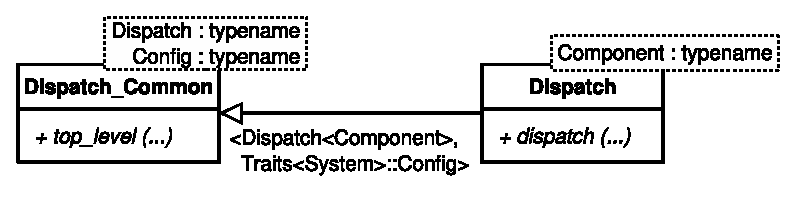
\includegraphics{fig/fig_dispatch_aspect}}
  }
  \subfloat[Component-specific dispatcher]{
         \label{fig_dispatch_aspect_comp}
         \begin{minipage}[c]{85mm}
         \centering
         \lstinputlisting[language=C++,style=prg,frame=single]{code/code_dispatch.cc}
         \end{minipage}
  }\\
  \subfloat[Specialization for a function-based entry-point]{         
         \label{fig_dispatch_aspect_cpp}
         \begin{minipage}[c]{79mm}
         \centering
         \lstinputlisting[language=C++,style=prg,frame=single]{code/code_dispatch_catapult_cpp.cc}
         \end{minipage}
  }\hspace{10mm}
  \subfloat[Specialization for a SystemC-based entry-point]{
         \label{fig_dispatch_aspect_sc}
         \begin{minipage}[c]{78mm}
         \centering
         \lstinputlisting[language=C++,style=prg,frame=single]{code/code_dispatch_catapult_sc.cc}
         \end{minipage}
  }
  \caption{Specialization of the dispatching aspect for different entry-point requirements}
  \label{fig_dispatch_aspect}
\end{figure*}

The actual implementation of the dispatching mechanism is implemented within the \emph{Dispatcher}
class. Since each component has a different method call interface, this class must be specialized
for each one. Static polymorphism is employed (Section
\ref{sec:proposal:unified_design:other}) so that the component-specific dispatching defined at
\emph{Dispatch} can be called from within \emph{Dispatch Common}. The binding between
\emph{Dispatch} and the desired specialization of \emph{Dispatch Common} is defined through a
system-wide \emph{Trait} class at the inheritance.

\subsubsection{Scenario definition}

The hardware scenario is defined by the \emph{HW Scenario} class and aggregates the static
allocation and dispatching aspects through multiple inheritance. The \emph{SW Scenario} class
aggregates only the allocation aspects using a \emph{metaprogrammed conditional inheritance}. This
is shown using the \condhwsw~notation in Figure \ref{fig_hw_sw_scenarios}, which
denotes that only one of the two generalizations occur at the same time. The code below shows how
the conditional inheritance is defined in the generic implementation of the \emph{SW scenario}:
%
\progcppinline{code_sw_scenatio}
%
The base aspect of the scenario is the result of the \emph{IF} metaprogram which depends on
static configurations defined in the component's \emph{Traits}.  The code sample below shows the
\emph{Trait} class used above, along with the implementation of the \emph{IF} metaprogram:
%
\progcppinline{code_trait_alloc_ifmeta}
%
In the specialization of \emph{Traits} for \emph{Component}, the configuration
\emph{static\_alloc} is equal to \emph{true}, in other words, static allocation will be used
instead of dynamic allocation when the software scenario is applied to \emph{Component}. The
\emph{IF} metaprogram that choses between possible options is implemented using C++ partial
template specialization. If \emph{condition} is \emph{true}, it defines \emph{Result} as the
type \emph{Then}. This is encoded in the base definition of the template. The template is
partially specialized for the false condition, defining \emph{Result} as the type \emph{Else}.

\subsubsection{Scenario adapter definition}

The scenario adapter incorporates the hardware/software aspects using conditional 
inheritance as well. The code sample below shows the generic declaration of the scenario adapter:
%
\progcppinline{code_scenario_adapter}
%
The adapter inherits the component behavior directly from its unified implementation,
while the base scenario is chosen by the \emph{IF} metaprogram according to the component's traits.
Components that can be implemented as either hardware or software have a trait named
\emph{hardware} that is used to define to which domain the component should be adapted. 

\subsubsection{Example: adapting the Scheduler}

This example illustrates how a component can be adapted using scenario adapters. Considering, for
instance, the scheduler case study, whose part of the base implementation (the \emph{unified
implementation}) is shown below:
%
\progcppinline{code_scheduler_base}
%
The \emph{insert}/\emph{remove} methods are responsible for insert/removing resources to/from the
scheduling queue. As described in Section \ref{sec:proposal:unified_design:hw_sw_sched}, in the
unified implementation, these methods expect to receive the externally allocated nodes. The code
sample below summarizes the definition of the scenario adapter for the scheduler:
%
\progcppinline{code_scheduler_adapter}
%
The adapter declaration follows the approach described previously: conditional inheritance to choose between the
scenarios and common inheritance to incorporate the unified implementation of the component. The
body of the scenario adapter implementation contains the necessary adaptations of the components
methods. The \emph{insert} and \emph{remove} methods of the \emph{Scheduler} class are redefined to
forward the allocation of nodes to the aspects. \emph{Scenario::allocate(obj,crit)} creates an
element for the scheduling list and receives as argument the object being scheduled and its
scheduling criterion. After the list element is created, it is obtained through
\emph{Scenario::get} and inserted in the scheduler. Depending on the configuration defined in
the scheduler's traits, \emph{Scenario::*} methods map to either \emph{HW Scenario} or \emph{SW
Scenario}, which inherits \emph{allocate}, \emph{get} and \emph{free} from the allocation aspects.

\subsection{Summary and discussion}

We have shown that a single C++ implementation can be used to generate both hardware and software
provided that it follows a careful design process. By careful design process, we mean a process that
assumes the later weaving of hardware/software dependencies using a scenario adapter. These
dependencies and their influence in the unified implementation are summarized below:\\
\textbf{Communication interface}: limiting the components interactions to method calls
allow the creation of a generic external mechanism (the dispatch aspect) that can be used by HLS
tools to infer the final hardware interface.\\
\textbf{Resource allocation:} components that require resource allocation can be designed in order
to
deal with links to the expected resources, as shown in the implementation of the lists in
Section \ref{sec:proposal:unified_design}. The actual allocation can then be performed externally
using the most suitable approach for the target domain.

In this work we have applied the concept of aspects and scenario adapters to introduce
hardware/software dependencies and implemented the mechanisms using C++ template metaprogramming.
However, other methods can be used for the same purpose. For instance, C's preprocessor macros (e.g.
\emph{\#define} and \emph{\#ifdef} blocks) allow one to introduce software- or
hardware-dependent code and to switch between different implementations. This a common
approach to distinguish executable from synthesizable C++ in current industrial designs.
Nevertheless, C++ templates offer two significant advantages over old-style C
macros: 1) macros are basically a text replacement mechanism and do not offer any kind of syntax
and
type checking, whereas templates are type-safe and its misuse generates compile-time errors; 2)
the implementation of a template can be partially or fully specialized to different types. Template
specialization is what in fact allows the metaprogrammed mechanisms shown in the previous sections.
Metaprogramming using C++ templates offers some disadvantages, however. Since templates are parsed
internally by the C++ compiler, debugging template metaprograms would require a debugger for the
C++ compilation process itself. One must rely only on source code analysis and error messages issued
by the compiler.

Another approach is to fully rely on mechanisms implemented in EDA tools to generate both hardware
and software from a single input model \cite{Schallenberg:2009, Keinert:2009, Rainer:2008}. Although
this usually provides a
more automated design flow, it creates a strong dependence between the source code and very specific
tools. Providing a systematic way to describe the semantics of the design process in the
source code level reduces such limitations. ANSI C++ and its OOP features are extensively supported
by hardware HLS tools and software compilers, thus increasing the applicability of our approach over
different design flows and tools.

It is also worth recalling that, as mentioned in Section \ref{sec:proposal:unified_design:other}, in
HLS, the design space can also be explored by using different synthesis directives (e.g. loop
unrolling/pipelining), yielding different implementations for the same C++ construct. Although we do
not deal with synthesis directives in this work, the techniques described in this paper can be used
to encode multiple sets of implementation options. For instance, directives defined using
\emph{pragmas}\footnote{the \emph{\#pragma} directive is the method specified by the C standard for
providing specific additional information to the compiler. It is platform and compiler dependent.}
can be specified within an aspect. Indeed, this aspect would have to be specialized for each
component, HLS tool, and intended hardware microarchitecture, since each of these would require a different
set of pragmas.

\section{Deployment of unified components}
\label{sec:implementation}

A uniform communication infrastructure is a requirement for design strategies in which the same
component can have different implementations in different domains. In this section we describe our
approach to support the seamless communication between hardware and software and the current
design flow used to deploy our unified components.

\subsection{Wrapping communication}
\label{sec:implementation:proxy_agent}

As discussed in Section \ref{sec:proposal:hw_sw_differences}, the component \emph{C2}, shown in the
OO model in Figure \ref{fig_oop_to_phy}, is an attribute of \emph{C1}. Considering that \emph{C1}
is the top-level in a HLS/compilation step, \emph{C2} would be compiled/synthesized together with
\emph{C1}. However, if the designer intends to have \emph{C1} and \emph{C2} as two independent
components implemented in different domains, then an additional mechanism is necessary. 

A way to overcome this issue is to use concepts from distributed object
platforms~\cite{Rincon:2009}. Figure \ref{fig_remote_invocation} illustrates \mbox{\emph{SW-->HW-->SW}}
interactions between components \emph{C1}, \emph{C2}, and \emph{C3}. The callee is represented in the domain of the
caller by a \emph{proxy}. When an operation is invoked on the components' proxy, the arguments
supplied are marshaled in a request message and sent through a \emph{communication channel} to the
actual component. In the \emph{HW-->SW} interaction, an \emph{agent} receives requests, unpacks
the arguments and performs local method invocations. The whole process is then repeated in the
opposite direction, producing reply messages that carry eventual return arguments back to the
caller. An \emph{agent} is not explicitly defined in the \emph{SW-->HW} interaction since the
\emph{dispatcher aspect} can already play its role for components in hardware.

\figSC{.6}{fig_remote_invocation}
{Communication between components in different domains (scenario adapters are omitted for simplicity)}

The implementation of
\emph{channels}, \emph{proxies} and \emph{agents} can be realized in several different ways. For
instance, when a bus-based communication channel is used, a proxy in hardware may be implemented as
slave device with memory mapped registers, and then notify the CPU through interrupt requests when
it has a request message ready to be read. Alternatively, on a \emph{Network-on-Chip}~(NoC) based
implementation, a packet-oriented interface would be used to transmit request messages. 

Such variability is related to choices regarding the hardware/software architecture of the chosen
implementation platform and should not affect the high-level components. Therefore, it is important
to separate the component-specific implementation that is part from the behavioral model from the
implementation related to artifacts of the underlying platform. Figure \ref{fig_remote_invocation}
also illustrates how we handle this separation of concerns. The platform-specific implementation of
\emph{HW\_Proxy} is encapsulated in the class \emph{HW\_Proxy\_Common}. \emph{HW\_Proxy\_Common} is
specialized for each platform following the same approach employed in the \emph{Dispatch} aspect (see
Figure \ref{fig_dispatch_aspect}). \emph{HW\_Proxy} then only defines the binding between the
component's interface methods with the marshaling operations defined by the specialized
\emph{HW\_Proxy\_Common}.


A key remaining issue is now how to make these mechanisms transparent within the components'
descriptions. An efficient solution is to use template metaprograms to replace the definition of a
component by its proxy only when necessary:
%
\progcppinline{code_component_map}
%
In the final implementation domain, \emph{C2} can be defined as an empty class that inherits from
its actual implementation depending on the configuration defined by \emph{C2}'s traits. In the
example above, the \emph{MAP} metaprogram selects between \emph{Scenario\_Adapter<C2>},
\emph{HW\_Proxy<C2>}, and \emph{SW\_Proxy<C2>}. \emph{MAP} uses the value of
\emph{Traits<System>::hardware\_domain} to determine if the code is being submitted to a HLS
tool or to a software compiler. If \emph{Traits<System>::hardware\_domain} is equal to
\emph{hardware}, which receives the value of \emph{Traits<C2>::hardware} in the example
above, then it must map to the actual implementation; therefore, \emph{Result} is equal to
\emph{Scenario\_Adapter<C2>} (\emph{Scenario\_Adapter<C2>} is also adapting C2's implementation
to the correct scenario). Otherwise, it maps to one of the proxies according to the current
implementation domain.


\subsection{A deployment platform}
\label{sec:implementation:platform}

In order to validate our mechanisms, we have assembled a platform for the deployment of our
unified components. Figure \ref{fig_platform2} shows the general structure of the chosen
hardware/software architecture. We rely on a NoC as the main communication link between hardware and
software components. The \textit{Real-time Star Network-on-Chip}~(RTSNoC)~\cite{Berejuck:2011} is
the core component of our SoC platform. RTSNoC consists of \emph{routers} with a star
topology that can be arranged forming a 2-D mesh. Each router has eight bidirectional channels that
can be connected to cores or to channels of other routers. Each hardware component is deployed as a
node connected to a router. Software components are compiled with an RTOS and run
in a \emph{CPU node} that consists of a softcore CPU and memories. The internal structure of CPU
nodes is based on the AXI4 family of protocols, which is becoming the industry's
standard for bus-based interconnection. In our current implementation we have relied on IPs
available at Opencores~\cite{OpenCores::2011}. Our current CPU node, for instance, is based on the
\emph{Plasma} softcore, an implementation of the MIPS32 ISA.

\figSC{.6}{fig_platform2}{System-on-Chip platform}

The software components run on EPOS~\cite{EPOS:2011}. EPOS provides the necessary run-time support
to implement the platform-specific concerns of proxies and agents.  A \emph{component manager}
handles communication between software and
hardware components and keeps lists of all existing proxies to hardware and agents to software. Each
component is associated to a unique ID that is mapped by a static resource table to a physical
address in the NoC. Upon a call request, this address is used to build packets containing the target
method ID and its arguments. These packets are sent through the NoC using the OS networking stack.
If the method has return values, the component manager blocks until it receives the return values
from the hardware component. 

On the hardware side, the entry-point defined by the \emph{dispatch aspect} (Section
\ref{sec:proposal:aspects}) blocks until a packet containing a method ID is received, followed by
packets containing the arguments. It parses the packets and performs the local method invocation,
sending back through the NoC eventual return values.

Packets sent to the CPU node trigger interrupts that are handled by an ISR defined by the
component manager. The ISR reads all pending packets and performs the necessary operations.
When the manager receives a packet containing return values, it searches a list of blocked proxies
and forwards the packet to the correct one. When a packet contains data from a method call request,
the information is forwarded to the respective agent. %The method dispatching of a software agent is
%very similar to the entry-point definition in the hardware dispatch aspect, but it receives data
%through successive explicit calls. Once all the data is received, the local call is performed in
%the software component.

\subsection{Design flow summary}
\label{sec:implementation:summary}

This work focuses only on general implementation guidelines and not on a whole design flow. Issues
such as design space exploration and design verification are not in the scope of this work.
Nevertheless, our mechanisms based on standard C++ solutions allow for a straightforward integration
with current synthesis tools and compilers. Figure~\ref{fig_adesd_flow_v2} shows
the steps we are currently using to go from C++ unified descriptions to components deployed in a
physical platform.

\figTC[ht]{.6}{fig_adesd_flow_v2}{Summary of the implementation flow}

The first steps show the artifacts of our proposed approach. Aspects, scenarios, and the unified
implementation of components made up the inputs for the implementation flows. Proxies and agents can
be automatically generated from the components' interface by a tool (EPOS's syntactical
analyzer~\cite{Schulter:2007} can be used to obtain the operation signatures of all components). The
final steps comprises the system generation. Once the hardware/software partitioning is
defined (by the components' Traits), the adapted components are fed to either the hardware or the
software generation flows. 

In the software flow, components are compiled along with the run-time support implemented in EPOS
using the GCC C++ compiler.
In the hardware flow, CatapultC is used to generate RTL descriptions. These descriptions are
bound with the hardware platform library and fed to the RTL synthesis tool. The platform library
contains the hardware IPs described in Section \ref{sec:implementation:platform}.

\section{Case study}
\label{sec:case_study}

In order to evaluate our approach, we have analyzed an industrial PABX application and designed some of its
basic building blocks using the proposed implementation guidelines.
The main component of the PABX system is a commutation matrix that switches connections amongst
different input/output data channels. These channels are connected to phone lines (through an AD/DA
converter), tone generators, and tone detectors. The system also supports the transmission of voice
data through an Ethernet network. Figure \ref{fig_pabx_soc_v3} shows the block diagram of the
digital part of the PABX system, with is deployed as a SoC in an FPGA.

\figSC{.55}{fig_pabx_soc_v3}{PABX SoC block diagram}

The components we have selected
to be reimplemented using unified C++ are highlighted and appear in as hardware and software, since
they can move between both domains depending on the final hardware/software partitioning. These
components are described in more detail below:\\
%
\textbf{EPOS's scheduler:} the case described in Section \ref{sec:proposal:unified_design}.\\
%
\textbf{ADPCM codec:} an IMA ADPCM encoder/decoder that performs data compression using an
\emph{adaptive differential pulse-code modulation}~(ADPCM) algorithm to convert 16-bit samples to
4-bit samples. The \emph{encode} and \emph{decode} operations are implemented in the same component
so they can share a local lookup table.\\
%
\textbf{DTMF detector:} the \textit{Dual-Tone Multi-Frequency}~(DTMF) detector receives signals
sampled from the phone lines connected to the central and detects DTMF tones. The entry point of the
original C implementation was a single function that received a pointer to a frame of samples and
returned the detected tone. The redesigned unified implementation defines two public operations:
\emph{add\_sample} updates a sample of the current frame; and \emph{do\_dtmf} performs the
detection. 


\subsection{Results}
\label{sec:case_study:results}

In order to demonstrate that unified implementations can be compared to dedicated ones in terms of
efficiency, we compare software scenario-adapted components against the original C
implementations (C++ for the scheduler), and hardware scenario-adapted components against
components manually tailored for high-level synthesis.

Figure \ref{fig_chart_sw}
compares the original software-only C (ADPCM and DTMF) and C++ (Scheduler) with the software
scenario-adapted C++. The footprints were obtained from the object files generated after compiling
each component in isolation, while the execution times were measured from the running application
using a time-stamp counter. Everything was compiled with \emph{gcc 4.0.2} targeting the MIPS32 ISA
and using \emph{level 2} optimizations. Figure \ref{fig_chart_sw_mem} shows an average increase of
about 4.9\% in the total memory footprint. In the case of the scheduler, the overhead can be
explained by the introduction of the \emph{option types} and the use of a more generic mechanism for
storage allocation (the \emph{Static/Dyn Alloc} aspect). For the remaining case studies, most of the
overhead comes from additional code required to encapsulate the behavior into more reusable OOP
classes with a clear method interface.

%Unified/HW-only
%Scheduler 1.056
%ADPCM 1.074
%DTMF 1.017
%\figSC{.75}{fig_chart_sw_mem}
%{Memory footprint of software-only C++ (SW-O) \emph{vs.}
%Unified C++ adapted to the software domain (U)}

%Unified/HW-only
%Scheduler 1.02
%ADPCM 1.03
%DTMF 1.05
%\tabSC[ht]{tab_result_sw_exec_time}
%{Execution time of software-only C++ \emph{vs.} unified C++}
%\figSC{.75}{fig_chart_sw_avg_time}{Normalized average execution times. Absolute values are shown
%above their respective bars.}

\begin{figure*}[htbp]
  \centering
  \subfloat[Memory footprint]{
      \label{fig_chart_sw_mem}
      \hspace{-5mm}
      \begin{minipage}[c]{59mm}
         \centering
         \scalebox{0.75}{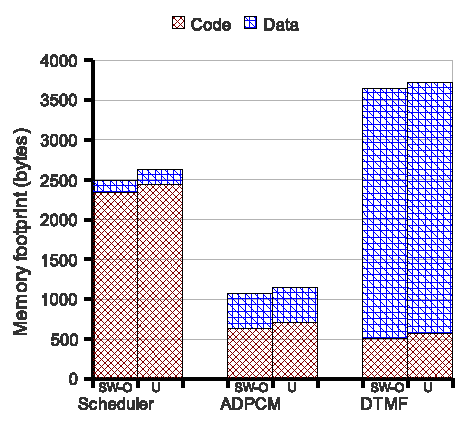
\includegraphics{fig/fig_chart_sw_mem}}
      \end{minipage}
  }
  \subfloat[Average and operations execution time]{
      \label{fig_chart_sw_avg_time}
      \begin{minipage}[c]{60mm}
         \centering
         \scalebox{0.75}{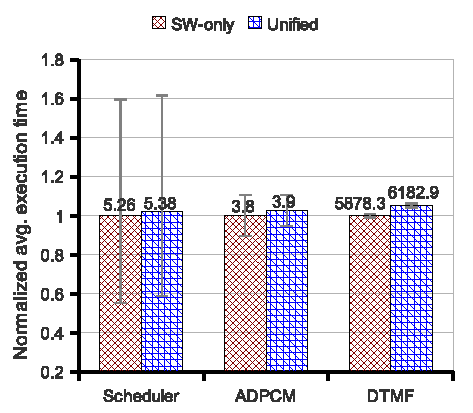
\includegraphics{fig/fig_chart_sw_avg_time}}
      \end{minipage}
      \begin{minipage}[c]{60mm}
         \generictablefontsize
         \centering
         \begin{tabular}{clrr}
\toprule
\multicolumn{2}{c}{\multirow{2}{*}{Component}}             & \multicolumn{2}{c}{Execution time ($\mu$s)} \\
\cmidrule(l){3-4}
                              &           & SW-only & Unified \\

\midrule
\multirow{5}{*}{Scheduler}    & insert    & ~~~6.0  & ~~~6.0 \\
                              & remove    & ~~~2.9  & ~~~3.3 \\
                              & suspend   & ~~~3.0  & ~~~3.1 \\
                              & resume    & ~~~6.0  & ~~~6.0 \\
                              & choose    & ~~~8.4  & ~~~8.5 \\
\midrule
\multirow{2}{*}{ADPCM}        & encode    & ~~~4.2  & ~~~4.2 \\                            
                              & decode    & ~~~3.4  & ~~~3.6 \\                            
\midrule
DTMF                          & do\_dtmf  & 5878.3  & 6182.9 \\
\bottomrule
\end{tabular}

%SW AVGs
%Memory footprint = 4.19 %
%Exec. time = 5.15 %


      \end{minipage}
  }
  \caption{Memory footprint (a) and execution time (b) of software-only C++ (SW-O) \emph{vs.}
           Unified C++ adapted to the software domain (U). The normalized average execution times 
           are plotted with absolute values above their respective bars.}
  \label{fig_chart_sw}
\end{figure*}

Figure \ref{fig_chart_sw_avg_time} shows the execution time
of each component operation and compare the average values. The execution time of the Scheduler and
the ADPCM codec is about 2.5\% higher in the unified implementation. The execution time of the
scheduler varies significantly according to the number of threads in the system (see error
bars in Figure \ref{fig_chart_sw_avg_time}). In this evaluation, we have experimented with 8 threads
and a round-robin scheduling criterion. For the DTMF detector, the
difference increases to 5\%. The original DTMF detector requires a single call to \emph{do\_dtmf} to
analyze a frame of samples, while the refactored DTMF detector requires several calls to
\emph{add\_sample} before performing the same task, which results in a more significant increase in
the execution time.

Table \ref{tab_result_hw_area} and Figures
\ref{fig_chart_hw_avg_area}--\ref{fig_chart_hw_results_speed_clks} compare the hardware
generated from unified C++ against hardware-only C++. \emph{Calypto's CatapultC UV 2011a} was used
to obtain RTL descriptions of the components. The descriptions were then synthesized using
\emph{Xilinx's ISE 13.4} targeting a \emph{Virtex6 XC6VLX240T} FPGA. CatapultC and ISE were
configured to minimize circuit area considering a target operating frequency of 100 MHz (the
operating frequency of the SoC).

%Unified/HW-only
%Scheduler 1.39
%ADPCM 1.27
%DTMF 0.97
\tabSC{tab_result_hw_area}
{FPGA synthesis results of hardware-only C++ \emph{vs.} unified C++}

\figSC{.75}{fig_chart_hw_avg_area}{Average FPGA resource utilization}
%\tabSCxXxXfigV[ht]
%{tab_result_hw_area}
%{fig_chart_hw_avg_area}{.75}
%{FPGA resource utilization of hardware-only implementations \emph{vs} Unified implementations
%adapted to the hardware domain}

\figSC{.75}{fig_chart_hw_results_speed_clks}{Performance of hardware components}


Table \ref{tab_result_hw_area} shows the amount of FPGA resources required for each
component and Figure \ref{fig_chart_hw_avg_area} plots the \emph{average resource utilization}. The
\emph{average resource utilization} is the arithmetic mean of the amount of each
specific resource weighted by its total amount available. This resulting value estimates the total
amount of FPGA area (in \%) required and is used as an area comparison metric. The results vary
significantly in each case study. The apparent smaller area of the unified DTMF detector is due to
different mapping of resources between \emph{RAM blocks} and \emph{flip-flops}, which resulted in 
smaller \emph{average resource utilization}. On the other hand, the unified Scheduler and ADPCM
require about 39\% and 27\% more area, respectively. Since the implementations of the HW-only and
unified ADPCMs are very similar, we conclude that, in this case, most of the extra area comes from
the \emph{Dispatch} aspect. The aspect implements a generic mechanism for parsing and issuing
operation requests, while the hardware-only descriptions focus on more specific and optimized
interfaces. This overhead can be considered significant and increases with the number of supported
operations. Nevertheless, this overhead is expected to be significantly reduced in future
implementations of \emph{Dispatch}. 

Figure \ref{fig_chart_hw_results_speed_clks} shows the maximum number of clock cycles required to perform an
operation. For the unified implementations of the Scheduler and the ADPCM, the \emph{agents'}
overhead is proportional to the number of arguments in the operation (2 for \emph{Scheduler::insert}
and 1 for \emph{ADPCM\_Codec::encode}). The high absolute overhead of the unified DTMF detector
comes from the several invocations of the \emph{add\_sample} method to fill its internal buffer.
This operation is implemented in a stream-like fashion in the HW-only detector.

To conclude our analysis, we have evaluated the total overhead of the communication infrastructure
required to handle transparent hardware/software communication. EPOS's internal components are
implemented using static metaprogramming to achieve high reusability with low overhead and its final
footprint depends on the application configuration. Therefore, it does not make sense to evaluate
certain components in isolation (e.g. the \emph{Component Manager}---Section
\ref{sec:implementation:platform}, which implements the runtime support). In order to
provide such evaluation, Table \ref{tab_soc_results} thus shows the total footprint considering the
following different partitionings of our PABX SoC: all the case studies are in software; all the
case studies are in hardware; and a hybrid partitioning in which only the scheduler is in software.
The values in the \emph{System} column are the total footprints subtracted by the footprints of all
case studies in the respective domain. For instance, the software footprint shown in the
\emph{System} column for a specific partitioning is the total software footprint subtracted by the
ones of all case studies implemented as software in that partitioning. This value allows us to
evaluate the overhead added by the component management mechanisms. %As reference, the footprints of
%the remaining hardware components are also provided in Table \ref{tab_result_hw_others_area}.
%\tabSC{tab_result_hw_others_area}
%{Hardware footprint of the remaining components}

%Entre parenteses o footprint total e do lado o total-footprint_componentes_individuais
\tabSC{tab_soc_results}
{SoC area footprint. In the hybrid partitioning, only the Scheduler is in software.}

%All SW - All HW = 4278 (Comp, mgm. + stubs ovehead when all SW)
%Hybrid - All HW = 126 
%Comp, mgm. + stubs ovehead (DTMF + ADPCM) = 4170
%About 4k + 30b per stub op
%----------
%About 1.3% more hardware area
As can be seen in Table \ref{tab_soc_results}, moving all cases to hardware reduced the total
footprint. By comparing the values in the \emph{System} column, we can see that, in the \emph{All
HW} partitioning,
the introduction of the component management mechanism added an overhead of 4278 bytes. By moving
the Scheduler back to software in the \emph{Hybrid} partitioning, the aforementioned overhead is
reduced to 4170 bytes. Considering the number of operations implemented in each proxy, we estimate
an initial overhead of about 4 Kbytes plus 30 bytes for each additional operation. We
expect to significantly reduce this overhead in future implementations, however, the current results
are acceptable if compared with similar infrastructures~\cite{Gracioli:2010}. On the hardware side,
the calculated area overhead when all cases are in hardware represents only 1.3\% of the total
circuit area and negligible when represented in terms of the total amount of resources available
in the target device (only 0.05\%).

\section{Conclusion}
\label{sec:conclusion}

In this paper we have explored a methodology based on AOP and OOP concepts in order to produce
unified descriptions of hardware and software components. We have shown that components designed
following the principles presented in this work are susceptible to both software and hardware
generation using standard compilers and HLS tools. This is possible through the isolation of
specific hardware and software characteristics (resource allocation and communication interface)
into aspect programs which are weaved with the unified descriptions only during the final stages of
the design process. 

The main contribution of this work is to show how the unified implementation of components, aspects,
and aspect weaving mechanisms can be implemented only using standard C++ and its metaprogramming
features. Therefore, the extraction of hardware/software implementation from the unified
implementation happens directly through language-level transformations, thus facilitating
compatibility with different C++-based HLS tools and design flows. We have demonstrated our methods
by redesigning some functional blocks of a PABX system. The resulting components confirmed that, at
an acceptable cost in area and performance, we can use C++ as a unified language to implement both
hardware and software in a straightforward way.

Our future works are twofold. As the comparison between hardware implementations suggests, new
features must be considered in order to provide a better support for high throughput data-oriented
applications. Our main concern with this aspect is on the seamless integration of stream-oriented
interfaces with our object-oriented modeling approach. Furthermore, though the
application of our design strategy to new cases, we also aim to identify new hardware/software
aspects that can be encapsulated using the proposed mechanisms.

%TODO apenas na vers�o final
%\section*{Acknowledgments}
%\addcontentsline{toc}{section}{Acknowledgments}
%The authors would like to thank Jo�o Pizani Flor and Marcelo Berejuck for providing the
%original implementation of the some of the case studies. This work is also partially supported by
%CAPES, under grants RH-TVD 006/2008 and 240/2008.

%\bibliographystyle{IEEEtran}
%\scriptsize

\bibliographystyle{IEEEtran}
\bibliography{paper}

%TODO apenas na vers�o final

%\vspace{-8mm}
%
%\begin{IEEEbiography}[{
\includegraphics[width=1in,height=1.25in,keepaspectratio]{fig/fig_bio_tiago}}]
%{Tiago Rog�rio M�ck}
%received his B.Sc. in Computer Science from the Federal University of Santa Catarina, Brazil. He is 
%currently a final year M.Sc. student in the Computer Science Department at the same university.
%His current research interests include computer architecture and embedded systems.
%\end{IEEEbiography}
%\vspace{-10mm}
%\begin{IEEEbiography}[{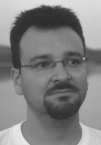
\includegraphics[width=1in,height=1.25in,keepaspectratio]{fig/fig_bio_guto}}]
%{Antonio Augusto Fr�hlich}
%received his Ph.D. in Computer Science from the Technical University of Berlin in 2001. He has been
%a professor in the Computer Science Department, Federal University of Santa Catarina, Brazil
%since 1995 and head of the Laboratory for Software and Hardware Integration since 2001. His current
%research interests include embedded systems and operating systems.
%\end{IEEEbiography}
%
%\vfill


\end{document}
